\documentclass[final, 5p, times, twocolumn, number, sort&compress]{elsarticle}

\usepackage{setspace}

\usepackage[colorlinks=true,allcolors=blue]{hyperref}
\usepackage[scaled=0.85]{roboto-mono}
\usepackage[T1]{fontenc}
\usepackage{listings}
\usepackage{textcomp}
\usepackage{xcolor}
\usepackage{xparse}
\usepackage{graphicx}
\usepackage{caption}
\usepackage{upgreek}
\usepackage{dcolumn}
\usepackage{amsmath}
\usepackage{amsfonts}
\usepackage{amssymb}
\usepackage{mathtools}
\usepackage{bm}
\usepackage{cuted}
\usepackage{braket}
\usepackage{orcidlink}
\usepackage{nicefrac}
\usepackage[ruled,vlined,linesnumbered]{algorithm2e}
\usepackage{booktabs}
\usepackage[online,referable]{threeparttablex}
\usepackage{tikz}
\usetikzlibrary{shapes.geometric, arrows.meta, positioning, shadows}
\usepackage{siunitx}
\sisetup{table-number-alignment=center,detect-weight=true,detect-inline-weight=math}
\usepackage{tabularx}

\usepackage{pythonhighlightcustom}

\DeclareMathOperator\G{G}

\newcommand{\ai}{\textit{ab initio}}
\newcommand{\eg}{\textit{e.g.}}
\newcommand{\etal}{\,\textit{et al.}}
\newcommand{\ie}{\textit{i.e.}}
\newcommand{\etc}{\textit{etc.}}

\newcommand{\speckit}{\texttt{SpecKit}}
\newcommand{\data}{\texttt{DeepFMKit.data}}
\newcommand{\physics}{\texttt{DeepFMKit.physics}}
\newcommand{\core}{\texttt{DeepFMKit.core}}
\newcommand{\fitters}{\texttt{DeepFMKit.fitters}}
\newcommand{\plotting}{\texttt{DeepFMKit.plotting}}
\newcommand{\fit}{\texttt{DeepFMKit.fit}}
\newcommand{\np}{\texttt{numpy}}
\newcommand{\sci}{\texttt{scipy}}
\newcommand{\plt}{\texttt{matplotlib}}
\newcommand{\cpp}{\texttt{C++}}

\begin{document}

% \doublespacing 

\journal{Computer Physics Communications}

\title{The \speckit{} python package: A toolkit for dynamic-resolution spectral analysis}

\author[1]{M.\ Dovale-\'Alvarez\orcidlink{0000-0002-6300-5226}\corref{cor}}\ead{mdovale@arizona.edu}
\author[2]{J.\ \'Alvarez-Vizoso\orcidlink{0000-0003-2879-2655}\corref{cor}}\ead{javizoso@aei.mpg.de}
\author[3]{G.\ Heinzel\orcidlink{0000-0003-1661-7868}\corref{cor}}\ead{gerhard.heinzel@aei.mpg.de}


\cortext[cor]{Corresponding author}

\affiliation[1]{
organization={James C.\ Wyant College of Optical Sciences, University of Arizona},
postcode={85721},
city={Tucson},
country={United States}
}

\affiliation[2]{
organization={Galicia Supercomputing Research Center (CESGA)},
postcode={15702},
city={Santiago de Compostela},
country={Spain}
}

\affiliation[3]{
organization={Max Planck Institute for Gravitational Physics (Albert Einstein Institute) and Leibniz Universit\"at Hannover, D-30167 Hannover, Germany},
postcode={30167},
city={Hannover},
country={Germany}
}

\begin{abstract}

We present \texttt{SpecKit}, a Python toolkit for dynamic-resolution spectral analysis of wideband signals spanning many decades in frequency, where high dynamic range and accurate calibration are required. \texttt{SpecKit} retains the standard Welch overlapped segmented averaging (WOSA) workflow, but replaces fixed resolution with a frequency scheduler that assigns, for each analysis frequency, a generally non-integer DFT bin index together with a segment length and overlap factor. This provides fine resolution at low frequencies while increasing the number of averages, reducing variance, toward high frequencies, without degrading calibration on logarithmic axes. The toolkit implements two schedulers: (i) ``LPSD'', which generates a quasi-logarithmic frequency grid by adapting segment lengths to maintain approximately constant relative bandwidth across frequencies, and (ii) ``LTF'', which extends LPSD with two practical controls: a minimum bin index to reduce low-frequency bias from window leakage, and a minimum DFT length to limit delay-induced distortions in cross-spectral estimates at high frequencies. The core implementation includes per-segment detrending, ENBW-based normalization, and a collection of useful window functions and optimal overlap factors, yielding reproducible power spectra or spectral densities with uncertainty estimates. Overall, \texttt{SpecKit} produces smooth, well-calibrated spectra on logarithmic frequency axes, avoids the variance trade-offs of fixed-resolution WOSA, and remains explicit about the per-bin resolution and averaging choices imposed by the scheduler. The package is open source and ships with tests and example scripts to support reproducibility and adoption in computational physics and engineering workflows.
%\bigskip
%\hrule
\bigskip

\begin{small}
\noindent
{\em Program Title:} SpecKit\\
{\em CPC Library link to program files:} (to be added by Technical Editor) \\
{\em Developer's repository link:} \href{https://github.com/mdovale/SpecKit}{github.com/mdovale/SpecKit}\\
{\em Licensing provisions:} BSD 3-clause \\
{\em Programming language:} Python 3.9 and higher \\
{\em Nature of problem:} Standard spectral estimation techniques, such as Welch's method, rely on the Fast Fourier Transform (FFT) with a fixed segment length, imposing a uniform frequency resolution across the spectrum. This is suboptimal for wideband physical signals spanning many decades, where logarithmic analysis is often required. Achieving high resolution at low frequencies necessitates long data segments, which severely limits the number of averages available to reduce statistical variance at high frequencies. This results in an inefficient trade-off between resolution and estimation stability. \\
{\em Solution method:} \speckit{} provides a high-performance, modular, and user-friendly Python library for dynamic-resolution spectral analysis. It replaces the fixed-resolution FFT with a flexible scheduling system that adapts segment lengths to approximate a logarithmic frequency axis, balancing resolution against statistical variance. It introduces a new scheduler algorithm, Logarithmic Transfer Function (LTF), which enforces constraints on minimum bin indices and segment lengths to mitigate windowing and time-delay biases. Computationally intensive kernels, including a generalized Goertzel algorithm and orthonormal polynomial detrending, are JIT-compiled via \texttt{Numba} to achieve C-like speeds while maintaining an accessible Python API. \\
\end{small}

\end{abstract}


\begin{keyword}
Spectral Analysis \sep 
Noise Estimation \sep 
Scientific Software \sep
Python
\end{keyword}


\maketitle


\section{Introduction}
\label{sec:introduction}

The estimation of a signal's power spectrum is a cornerstone of signal processing and data analysis, with wide-ranging applications in experimental physics, engineering, communications, and astronomy. While the Fast Fourier Transform (FFT) provides an efficient algorithm for computing the Discrete Fourier Transform (DFT), the resulting raw periodogram is known to be an inconsistent estimator of the true power spectrum, exhibiting high variance that does not decrease as the signal length increases~\cite{Oppenheim1999}.

To overcome this limitation, the Welch Overlapped Segment Averaging (WOSA) method is a widely adopted technique~\cite{Welch1967}. It mitigates the variance of the periodogram by dividing the signal into overlapping segments, applying a window function to each segment to reduce spectral leakage, and then averaging the periodograms computed from each segment. A fundamental characteristic of the standard WOSA method, as implemented in ubiquitous scientific libraries such as \sci{}~\cite{SciPy}, is its fixed frequency resolution, $\Delta f = f_s/L$, where $f_s$ is the sampling frequency and $L$ is the uniform length of each segment. This imposes a rigid trade-off between spectral resolution and statistical variance. High resolution (large $L$) is achieved at the cost of having fewer segments to average, leading to noisy estimates with high variance. Conversely, reducing variance by increasing the number of averages (small $L$) degrades the ability to resolve fine spectral features.

This trade-off becomes particularly restrictive for wideband signals whose features span many decades and are naturally analyzed on a logarithmic frequency axis. A fixed $\Delta f$ is highly inefficient in this context: at high frequencies, the resolution is often excessively fine, resulting in unnecessarily high variance, while at low frequencies, it is often too coarse to resolve important physical phenomena. To address this, Tr\"obs and Heinzel introduced a dynamic-resolution approach that adapts the WOSA method for logarithmic frequency axes~\cite{Troebs2006}. Their Logarithmic Power Spectral Density (LPSD) algorithm replaces the fixed segment length with a frequency-dependent one, determined by a sophisticated scheduling procedure. The scheduler generates a quasi-logarithmic frequency grid that provides fine resolution at low frequencies while systematically increasing the number of averages (and thus reducing variance) at high frequencies.

This paper presents \speckit{}, a modern, high-performance, open-source Python implementation of this dynamic-resolution paradigm. While the foundational LPSD algorithm provides an excellent solution for logarithmic spectral estimation, \speckit{} introduces a significant extension, which we term the Logarithmic Transfer Function (LTF) algorithm. The LTF scheduler builds upon the LPSD framework by incorporating two new control parameters to address critical issues in practical data analysis. First, it introduces a minimum bin number, $b_{\min}$, to formally mitigate the known bias in the lowest-frequency bins of a windowed periodogram caused by power aliasing from negative frequencies---a phenomenon noted in~\cite{Troebs2006} and~\cite{Heinzel2002TN}. Second, it enforces a minimum segment length, $L_{\min}$, which is crucial for preserving the integrity of cross-spectral estimates (\eg, transfer functions and coherence) in the presence of relative time delays between signals.

\speckit{} is engineered as a comprehensive and accessible toolkit. Its high-performance core, accelerated with Numba~\cite{Numba}, implements per-segment polynomial detrending and utilizes the Goertzel algorithm~\cite{Goertzel1958} for efficient computation at the arbitrary non-integer bin numbers required by the scheduler. The result is a seamless, well-calibrated spectrum on a logarithmic axis, free from the stitching artifacts and suboptimal variance distribution of fixed-resolution methods. In this paper, we detail the theory behind the dynamic-resolution WOSA method and the novel LTF scheduler, describe the software architecture, and demonstrate its utility through a series of illustrative applications.



\subsection{Comparison to Existing Software}
\label{sec:existing-software}

The landscape of spectral analysis software can be broadly divided into standard, fixed-resolution tools and specialized, dynamic-resolution libraries.

The industry standards for fixed-resolution analysis are the \texttt{pwelch} function in the MATLAB Signal Processing Toolbox~\cite{MATLAB} and the \texttt{scipy.signal.welch} function in the Python \sci{} library~\cite{SciPy}. These are robust, highly optimized, and well-documented tools suitable for a vast range of applications. However, as discussed, they are based on a fixed-segment-length WOSA implementation and do not natively support the dynamic-resolution approach required for optimal logarithmic spectral estimation.

Within the specialized domain of LPSD/LTF-type algorithms, two notable prior implementations exist. The LISA Technology Package Data Analysis (\texttt{LTPDA}) toolbox~\cite{Hewitson2009, HewitsonLTPDA} is a comprehensive MATLAB-based suite developed for the gravitational-wave community. First released in 2007, it was an early adopter of the LPSD/LTF algorithms and has been historically significant within its field. However, it has not been updated since 2017 and can be considered legacy software, exhibiting compatibility issues with modern MATLAB versions. Its nature as a large, multi-purpose library also makes it difficult to maintain and integrate into modern, modular Python workflows~\cite{python-language-reference}.

The second is the original \texttt{LPSD-C} implementation written in the C language by the algorithm's progenitors, Heinzel and Tr\"obs~\cite{LPSDC}. This version is exceptionally fast but was developed for internal use, is not publicly available, and lacks documentation and long-term maintenance.

\speckit{} is designed to fill the gap left by these implementations. It provides the first open-source, actively maintained, and thoroughly documented Python package dedicated to dynamic-resolution spectral analysis. It aims to match the performance of the original C code through JIT compilation with Numba, while offering the accessibility, ease of use, and ecosystem integration of a modern Python library. By focusing specifically on spectral analysis, it avoids the large, complex structure of \texttt{LTPDA}, providing a lightweight and maintainable tool for the broader scientific and engineering community.


\subsection{Structure of the Paper}
\label{sec:structure}

This paper is structured as follows. Section~\ref{sec:theory} presents the mathematical framework underlying the dynamic-resolution WOSA method, including the LPSD and LTF scheduling algorithms. Section~\ref{sec:architecture} describes the software architecture and design principles of \speckit{}. Section~\ref{sec:math-engine} details the high-performance mathematical kernels, including the generalized Goertzel algorithm and orthonormal polynomial detrending, and presents performance benchmarks comparing \speckit{} to MATLAB \texttt{LTPDA}. Section~\ref{sec:schedulers} provides a comparative analysis of the different scheduling algorithms available in the package. Sections~\ref{sec:application-1} through~\ref{sec:application-3} present three illustrative applications: the impact of window function selection on high-dynamic-range signals, the quantification of time-delay bias errors in cross-spectral estimates, and optimal spectral analysis for Multi-Input Single-Output (MISO) systems. Section~\ref{sec:verification} discusses the software testing strategy and code availability. Finally, Section~\ref{sec:summary-and-outlook} summarizes the contributions and outlines future development directions. The appendices provide reference tables for spectral quantities and class diagrams illustrating the software architecture.    


\section{Theory}
\label{sec:theory}

The core of the \speckit{} library is a generalization of the Welch Overlapped Segment Averaging (WOSA) method. While the classical approach employs a fixed resolution for all frequencies, our method uses a frequency-dependent resolution, which requires a scheduling algorithm to generate an optimized frequency plan. In this section, we first present the definitive mathematical framework of the dynamic-resolution WOSA method. We then describe the Logarithmic Power Spectral Density (LPSD) scheduler, which generates a quasi-logarithmic frequency grid, followed by our novel Logarithmic Transfer Function (LTF) scheduler, which extends the LPSD algorithm to address practical challenges in experimental data analysis.

\subsection{The Generalized WOSA Method}
\label{sec:wosa}

Consider a time series of $N$ equidistant samples, $x(n)$ for $n=0, \dots, N-1$, recorded with a sampling frequency $f_s$. We aim to compute spectral estimates at a set of $J$ discrete Fourier frequencies, $f(j)$ for $j=0, \dots, J-1$. Unlike the standard FFT-based approach, this set of frequencies is not required to be linearly spaced. For each frequency $f(j)$, the analysis proceeds as follows.

First, the data record is divided into $K(j)$ overlapping segments, each of length $L(j)$. The starting points of these segments are $D(j)$ samples apart, such that the data of segment $k$ is given by $\{ x(l + k \cdot D(j)),\,l=0,\dots,L(j)-1 \}$. Note that the key parameters $L(j)$, $K(j)$, and $D(j)$ are all functions of the analysis frequency index $j$.

Each segment is optionally de-trended. By default, the mean value is subtracted to perform a zero-order de-trending,
\begin{equation}
a(j,k) = \frac{1}{L(j)} \sum \limits_{l=0}^{L(j)-1} x(l + k \cdot D(j)),
\end{equation}
which mitigates spectral leakage from the DC component. We then form the windowed sequences,
\begin{equation}
G(j,k,l) = \left[ x(l + k \cdot D(j)) - a(j,k) \right] w(j,l),
\end{equation}
where $w(j,l)$ is a data window selected to reduce spectral leakage from tones that do not fall exactly on a frequency bin. A typical choice is the Hann window, defined as
\begin{equation}
w(j,l) = \frac{1}{2}\left[ 1- \cos \left( \frac{2 \pi l}{L(j)} \right) \right].
\end{equation}
A comprehensive review of window functions is given in~\cite{Heinzel2002TN}. Next, we compute the scalar products of these sequences with the complex exponential of the corresponding Fourier frequency. Mathematically, this corresponds to the Discrete Fourier Transform (DFT) of $G(j,k,l)$ at a single, potentially non-integer, bin number $m(j)$. While standard FFT algorithms require integer bin numbers, we evaluate this sum using the Goertzel algorithm (see Section~\ref{sec:math-engine}) to support arbitrary frequency resolution:
\begin{equation}
A(j,k) = \sum \limits_{l=0}^{L(j)-1} G(j,k,l) \exp \left( -2\pi i \frac{m(j) \cdot l}{L(j)} \right),
\end{equation}
where the bin number $m(j)$ is defined as the ratio of the analysis frequency to the resolution bandwidth, $r(j)$:
\begin{equation}
m(j) = \frac{f(j)}{r(j)}.
\label{equation:bin-number}
\end{equation}
The resolution bandwidth, which represents the width of a single DFT bin, is itself governed by two fundamental relationships. First, it is determined by the segment duration in time:
\begin{equation}
r(j) = \frac{f_s}{L(j)}.
\label{equation:r_fs_Lj}
\end{equation}
Second, in our dynamic-resolution framework, we enforce the condition that the resolution bandwidth should match the local spacing of the frequency grid:
\begin{equation}
r(j) = f(j + 1) - f(j).
\label{equation:r_Dfj}
\end{equation}
Equation~\ref{equation:r_fs_Lj} ensures that the spectral estimate is physically meaningful, while Eq.~\ref{equation:r_Dfj} maintains the property of the original WOSA method that adjacent frequency bins are approximately independent. If $f(j+1)-f(j) \gg r(j)$, spectral features could be missed between bins. Conversely, if $f(j+1) - f(j) \ll r(j)$, adjacent bins would contain highly correlated, redundant information.

Finally, we obtain the squared magnitudes of the complex scalar products, $|A(j,k)|^2$, and form the spectral estimate at the frequency $f(j)$ by averaging over all $K(j)$ segments:
\begin{equation}
P(f(j)) = \frac{C(j)}{K(j)} \sum \limits_{k=0}^{K(j)-1} |A(j,k)|^2.
\end{equation}
Here, $C(j)$ is a frequency-dependent calibration coefficient used to scale the result to a power spectrum (PS) or a power spectral density (PSD). The coefficient for a one-sided power spectrum is given by
\begin{equation}
C_{\rm PS} (j) = \frac{2}{\left( \sum\limits_{l=0}^{L(j)-1} w(j,l) \right)^{2}},
\end{equation}
and the corresponding coefficient for a one-sided power spectral density is
\begin{equation}
C_{\rm PSD} (j) = \frac{2}{f_s \sum\limits_{l=0}^{L(j)-1} w^2(j,l)}.
\end{equation}
The factor of 2 accounts for the power from the negative frequencies that is folded into the positive frequency axis.

\subsection{The LPSD Scheduler}
\label{sec:lpsd}
The Logarithmic Power Spectral Density (LPSD) scheduler, first presented in~\cite{Troebs2006}, is an algorithm designed to generate the frequency plan---the set of tuples $\{f(j), r(j), L(j), K(j)\}$---used by the generalized WOSA method. Its primary goal is to create a frequency grid that approximates a logarithmic spacing, which is often preferable for analyzing wideband signals.

An ideal logarithmic frequency grid is a geometric progression, which implies that the frequency spacing, or resolution, is directly proportional to the frequency itself: $r(j) \propto f(j)$. This defines a constant-Q (Quality factor) analysis, where $Q = f(j)/r(j)$ is constant across the spectrum. This contrasts with standard FFT-based methods, which operate with a constant bandwidth $r = f_s/L$ and thus have a Q-factor that increases linearly with frequency.

The LPSD scheduler approximates a constant-Q analysis by first defining an ideal logarithmic scaling factor, $c_{\log}$, derived from the total number of available frequency bins ($N/2$) and the desired number of output frequencies, $J_{\rm des}$:
\begin{equation}
    c_{\log} = \left(\frac{N}{2}\right)^{\frac{1}{J_{\rm des}}} - 1.
    \label{equation:clog}
\end{equation}
The ideal resolution for the scheduler, which we denote $r'(j)$, is then calculated as:
\begin{equation}
    r'(j) = f(j) \cdot c_{\log}.
    \label{equation:ideal_r_lpsd}
\end{equation}
However, strictly adhering to this ideal is often physically impossible or statistically undesirable. Any time series of length $N$ has a fundamental resolution limit, $r_{\min}$, determined by its total duration:
\begin{equation}
    r(j) \ge \frac{f_s}{N} \equiv r_{\min}.
\end{equation}
Furthermore, to ensure statistical stability, it is desirable to have a minimum number of averages, $K_{\text{des}}$. This imposes a second constraint, defining a resolution threshold, $r_{\text{avg}}$, which corresponds to the coarsest resolution that guarantees at least $K_{\text{des}}$ averages with a given fractional overlap $\xi$:
\begin{equation}
    r_{\text{avg}} = r_{\min} \cdot \left( 1 + (1-\xi)(K_{\text{des}}-1) \right).
\end{equation}
The LPSD algorithm generates the frequency grid iteratively, employing a three-regime heuristic at each step to determine the next resolution. The procedure starts at $f(j=0)=f_s/N$ and proceeds as follows: for the current frequency $f(j)$, it calculates the ideal resolution $r'(j)$ using Eq.~\ref{equation:ideal_r_lpsd}. It then determines the compromise resolution, $r''(j)$, based on which of three regimes $r'(j)$ falls into:
\begin{equation}
    r''(j) =
    \begin{cases}
    r'(j), & \text{if } r'(j) \geq r_{\text{avg}} \\
    \sqrt{r_{\text{avg}} \cdot r'(j)}, & \text{if } r_{\min} \leq r'(j) < r_{\text{avg}} \\
    r_{\min}, & \text{if } r'(j) < r_{\min}
    \end{cases}
    \label{eq:lpsd_heuristic}
\end{equation}
In the high-frequency regime ($r'(j) \geq r_{\text{avg}}$), the ideal logarithmic spacing is achievable. In the low-frequency regime ($r'(j) < r_{\min}$), the physical limit is enforced, resulting in linear spacing. In the transition regime, the geometric mean is used as a heuristic compromise. From this compromise resolution, the final integer segment length $L(j)$ is calculated, which in turn defines the final, practical resolution $r(j) = f_s/L(j)$. The next frequency in the grid is then given by $f(j+1) = f(j) + r(j)$, and the process repeats.

\subsection{The LTF Scheduler}
\label{sec:ltf}
The Logarithmic Transfer Function (LTF) algorithm is a novel extension of the LPSD scheduler, designed to address two practical issues that arise at the low and high ends of the spectrum. It introduces two additional control parameters, $b_{\min}$ and $L_{\min}$, to provide more robust spectral estimates in real-world applications. The original LPSD algorithm can be considered a special case of LTF with the default parameters $b_{\min}=1$ and $L_{\min}=1$.

\subsubsection{Low-Frequency Windowing Bias Correction}
As is well known, windowing data segments to reduce spectral leakage introduces a bias in the lowest frequency bins of a one-sided spectrum~\cite{Heinzel2002TN}. This bias results from power aliasing from negative frequency bins, which is not eliminated by subtracting the segment mean. The number of affected bins depends on the spectral window used; specifically, the effective half-width of the window's transfer function determines the first bin that can be considered unbiased.

The LTF algorithm addresses this with the control parameter $b_{\min}$, which sets the minimum permissible bin number. The scheduler's logic, described in Algorithm~\ref{alg:ltf}, is modified in two ways. First, the entire frequency grid generation starts at a higher minimum frequency, $f_{\min} = b_{\min} \cdot (f_s/N)$, effectively ignoring the region most susceptible to bias. Second, during the iterative process, after the compromise resolution $r''(j)$ has been calculated using Eq.~\ref{eq:lpsd_heuristic}, a check is performed. If the resulting bin number, $m(j) = f(j)/r''(j)$, is less than $b_{\min}$, the bin number is clamped to $b_{\min}$ and the resolution is recalculated as $r''(j) = f(j)/b_{\min}$. This ensures no frequency bin in the final output has a bin number smaller than the specified limit.

\subsubsection{High-Frequency Delay Bias Correction in Multi-Channel Applications}
When computing cross-spectra between two channels, a relative time delay between the signals can cause significant distortion in the estimate. This issue becomes acute when the length of the DFT segments, $L(j)$, becomes comparable to or shorter than the delay. The LPSD algorithm is particularly prone to this at high frequencies, where it naturally uses many averages of very short segments to maintain a coarse, logarithmic-like spacing.

As a practical remedy, the LTF algorithm introduces a second control parameter, $L_{\min}$, which defines the minimum allowable segment length. The implementation is a straightforward clamp: after the algorithm calculates the required segment length $L(j)$ for a given frequency $f(j)$, if $L(j) < L_{\min}$, it is set to $L_{\min}$.

The consequence of enforcing this minimum length is a modification to the frequency grid at the high end of the spectrum. Since the resolution is inversely proportional to the segment length ($r(j) = f_s/L(j)$), forcing $L(j)$ to be larger than it otherwise would be results in a frequency resolution $r(j)$ that is finer. This means that at high frequencies where this constraint is active, the frequency bins will be spaced more densely than the ideal logarithmic spacing would require. This is a deliberate trade-off, sacrificing perfect logarithmic spacing to ensure the integrity of cross-spectral estimates. A detailed, step-by-step implementation of the full LTF scheduling procedure is provided in Algorithm~\ref{alg:ltf}.

\begin{algorithm}[ht!]
\small
\caption{The LTF Scheduler}
\label{alg:ltf}

\KwIn{$N, f_s, \xi, b_{\min}, L_{\min}, J_{\text{des}}, K_{\text{des}}$}
\KwOut{Frequency plan $\{f_j\}, \{r_j\}, \{m_j\}, \{L_j\}, \{K_j\}, \{D_j\}, \{O_j\}$}

\tcc{Phase 1: Initialize constants}
$x_{\text{ov}} \gets 1 - \xi$\;
$f_{\min} \gets b_{\min} \cdot f_s / N$\;
$f_{\max} \gets f_s / 2$\;
$r_{\min} \gets f_s / N$\;
$r_{\text{avg}} \gets r_{\min} \cdot (1 + x_{\text{ov}}(K_{\text{des}} - 1))$\;
$c_{\log} \gets (N/2)^{1/J_{\text{des}}} - 1$\;

\tcc{Phase 2: Scheduler loop}
$j \gets 0$; $f_j \gets f_{\min}$\;

\While{$f_j < f_{\max}$}{
  $r' \gets f_j \cdot c_{\log}$ \tcp*{Ideal log resolution}

  \tcc{Apply three-regime heuristic}
  \uIf{$r' \ge r_{\text{avg}}$}{
    $r'' \gets r'$ \;
  }
  \uElseIf{$\sqrt{r_{\text{avg}} \cdot r'} > r_{\min}$}{
    $r'' \gets \sqrt{r_{\text{avg}} \cdot r'}$ \;
  }
  \Else{
    $r'' \gets r_{\min}$ \;
  }

  \If{$f_j / r'' < b_{\min}$}{
    $r'' \gets f_j / b_{\min}$ \tcp*{Enforce min bin number}
  }

  $L_j \gets \text{round}(f_s / r'')$\;

  \If{$L_j > N$}{ $L_j \gets N$ }
  \If{$L_j < L_{\min}$}{ $L_j \gets L_{\min}$ \tcp*{Enforce min length} }

  $K_j \gets \text{round}((N - L_j) / (x_{\text{ov}} \cdot L_j) + 1)$\;

  \If{$K_j = 1$}{ $L_j \gets N$ }

  $r_j \gets f_s / L_j$ \tcp*{Recalc exact resolution}
  $m_j \gets f_j / r_j$\;
  
  Store $f_j, r_j, m_j, L_j, K_j$\;

  $f_{j+1} \gets f_j + r_j$ \tcp*{Step by bin width}
  $j \gets j + 1$\;
}
$J \gets j$\;

\tcc{Phase 3: Post-processing (Start Indices)}
\For{$j \gets 0$ \KwTo $J-1$}{
    \eIf{$K_j = 1$}{
        $D_j \gets [0]$; $O_j \gets 0$\;
    }{
        $S \gets (N - L_j) / (K_j - 1)$ \tcp*{Shift}
        $D_j \gets [\text{round}(k \cdot S) \text{ for } k \in 0..K_j-1]$\;
        $O_j \gets \text{mean}((L_j - (D_{j}[1:] - D_{j}[:-1]))/L_j)$\;
    }
}
\end{algorithm}



\subsubsection{The Vectorized LTF Scheduler for Improved Performance}
\label{sec:vectorized-ltf}

While the iterative approach of the LTF scheduler described in Algorithm~\ref{alg:ltf} is a direct implementation of the underlying theory, its sequential nature, when executed in an interpreted language like Python, can become a computational bottleneck for plans with a large number of desired frequencies ($J_{\rm des}$). To address this, \speckit{} provides a high-performance, vectorized variant of the algorithm that yields a nearly identical frequency plan in a fraction of the time.

This approach, detailed in Algorithm~\ref{alg:vectorized-ltf}, decouples the calculation of parameters from the generation of the final frequency plan by operating in two main phases:
\begin{enumerate}
    \item \textbf{Pre-computation phase:} Instead of calculating parameters one frequency at a time, the algorithm first creates a dense, logarithmically spaced grid of candidate frequencies spanning the entire analysis band. The complete LTF compromise logic---including the three-regime heuristic and the clamping rules for $b_{\min}$ and $L_{\min}$---is then applied to this entire grid at once using efficient array operations in NumPy~\cite{Harris2020}. This produces a set of ``parameter maps'' (\eg, $r_{\text{map}}$, $L_{\text{map}}$) that store the correct, final analysis parameters for any frequency within the dense grid.
    \item \textbf{Selection phase:} A fast ``walker'' loop then generates the final frequency plan. It starts at $f_{\min}$ and, at each step, performs a fast lookup into the pre-computed parameter maps to find the definitive resolution for the current frequency. It then takes a step of that exact size to determine the next frequency, perfectly satisfying the condition $f(j+1) = f(j) + r(j)$.
\end{enumerate}
This method trades a modest increase in memory usage for a significant reduction in computation time. The use of a discrete, pre-computed grid means the output is a high-fidelity approximation of the iterative method, with minor numerical differences that are negligible in practice. Due to its superior performance, this vectorized scheduler is the default in \speckit{}.


\begin{algorithm}[ht!]
\small
\caption{The Vectorized LTF Scheduler}
\label{alg:vectorized-ltf}

\KwIn{$N, f_s, \xi, b_{\min}, L_{\min}, J_{\text{des}}, K_{\text{des}}$}
\KwOut{Frequency plan $\{f_j\}, \{r_j\}, \{L_j\}, \dots$}

\tcc{Phase 1: Pre-computation (Vectorized)}
Generate dense, log-spaced grid $f_{\text{grid}}$ from $f_{\min}$ to $f_{\max}$\;
$r'_{\text{grid}} \gets f_{\text{grid}} \cdot c_{\log}$\;

\tcc{Apply heuristic vectorially}
$r''_{\text{grid}} \gets r_{\min} \cdot \mathbf{1}$\;
mask1 $\gets (r'_{\text{grid}} \ge r_{\text{avg}})$\;
$r''_{\text{grid}}[\text{mask1}] \gets r'_{\text{grid}}[\text{mask1}]$\;
mask2 $\gets (r_{\min} \le r'_{\text{grid}}) \land (r'_{\text{grid}} < r_{\text{avg}})$\;
$r''_{\text{grid}}[\text{mask2}] \gets \sqrt{r_{\text{avg}} \cdot r'_{\text{grid}}[\text{mask2}]}$\;

\tcc{Apply constraints vectorially}
mask\_b $\gets (f_{\text{grid}} / r''_{\text{grid}} < b_{\min})$\;
$r''_{\text{grid}}[\text{mask\_b}] \gets f_{\text{grid}}[\text{mask\_b}] / b_{\min}$\;

$L_{\text{map}} \gets \text{round}(f_s / r''_{\text{grid}})$\;
$L_{\text{map}} \gets \text{clip}(L_{\text{map}}, L_{\min}, N)$\;
$K_{\text{temp}} \gets \text{round}((N - L_{\text{map}}) / (x_{\text{ov}} L_{\text{map}}) + 1)$\;
$L_{\text{map}}[K_{\text{temp}} = 1] \gets N$\;

$r_{\text{map}} \gets f_s / L_{\text{map}}$\;

\tcc{Phase 2: Selection (Walker)}
$j \gets 0$; $f_j \gets f_{\min}$\;
\While{$f_j < f_{\max}$}{
  idx $\gets$ \text{searchsorted}($f_{\text{grid}}, f_j$)\;
  
  $r_{\text{sel}} \gets r_{\text{map}}[\text{idx}]$\;
  $L_{\text{sel}} \gets L_{\text{map}}[\text{idx}]$\;
  $K_{\text{sel}} \gets K_{\text{map}}[\text{idx}]$\;
  Store $f_j, r_{\text{sel}}, L_{\text{sel}}, K_{\text{sel}}$\;

  $f_{j+1} \gets f_j + r_{\text{sel}}$\;
  $j \gets j + 1$\;
}

\tcc{Phase 3: Post-processing (Vectorized)}
$S \gets (N - L) / (K - 1)$ where $K > 1$\;
$D_j \gets \text{round}(\text{arange}(K_j) \cdot S_j)$\;
$O_j \gets (L_j - S_j) / L_j$\;
\end{algorithm}

\section{Software Architecture}
\label{sec:architecture}

\begin{figure}
\centering
\begin{python}
from speckit import compute_spectrum
import matplotlib.pyplot as plt
# --- 1. Load time series data ---
fs = 2.0  # Sampling frequency in Hertz
x = np.random.rand(int(2e6))  # Random data
# --- 2. Calculate spectrum ---
obj = compute_spectrum(
    x,
    fs,
    order=0,    # Detrending order
    win="Hann", # Window function
    olap=0.75,  # Fractional overlap
)
# --- 3. Plot amplitude spectral density ---
ax = obj.plot(which="asd", errors=True, sigma=3)
plt.show()
\end{python}
\caption{\speckit{}'s basic workflow.}
\label{fig:workflow}
\end{figure}

\speckit{} is designed with a modular architecture that separates the definition of the spectral analysis parameters from the heavy numerical computation. This design pattern, often referred to as a configuration-computation separation, allows for rigorous validation of the analysis plan before any expensive data processing occurs. The package is organized into four primary modules:

\begin{enumerate}
    \item \textbf{Analysis API (\texttt{analysis.py}):} This module exposes the high-level \texttt{SpectrumAnalyzer} class. It serves as the primary user interface, handling input validation, window function selection, and the coordination of the scheduling and computation phases. It also defines the \texttt{SpectrumResult} container, an immutable data structure that provides lazy evaluation of derived spectral quantities (\eg, coherence, transfer functions, and error estimates) from the core sufficient statistics.
    
    \item \textbf{Schedulers (\texttt{schedulers.py}):} This module contains the implementations of the frequency planning algorithms, including the iterative LPSD, the iterative LTF, and the vectorized LTF schedulers. These functions are pure: they accept configuration parameters and return a dictionary defining the exact frequency and segmentation plan (frequencies, bin numbers, segment lengths, starting indices, and overlap factors).
    
    \item \textbf{Mathematical Core (\texttt{core.py}):} The numerical heavy lifting is isolated in this module. It contains Just-In-Time (JIT) compiled kernels for the Goertzel algorithm, polynomial detrending, and windowing. These kernels are written to be compatible with \texttt{Numba}~\cite{Numba}, allowing them to bypass the Python Global Interpreter Lock (GIL) and achieve C-like performance through automatic parallelization across data segments.
    
    \item \textbf{Utilities and Visualization:} Helper modules for signal generation (\texttt{noise.py}), signal processing (\texttt{dsp.py}, with fractional delay in \texttt{lagrange.py}), window function definitions (\texttt{flattop.py}), and publication-quality plotting (\texttt{plotting.py}).
\end{enumerate}

The typical workflow involves instantiating a \texttt{SpectrumAnalyzer} with the time-series data and desired configuration (\eg, window type, overlap, detrending order). The analyzer then generates a ``plan'' using the selected scheduler. This plan is passed to the computation engine, which executes the parallelized kernels to produce a \texttt{SpectrumResult}.

\begin{figure}
\centering
\includegraphics[scale=1]{fig01.pdf}
\caption{Comparison of Amplitude Spectral Density (ASD) estimated via \speckit{} and \texttt{scipy.signal.welch} for a random noise signal consisting of $2 \times 10^6$ samples sampled at $f_s=2$\,Hz. The shaded region indicates the $\pm 3\sigma$ confidence interval derived from the \speckit{} empirical variance estimates. The plot illustrates the advantage of the dynamic-resolution approach: at high frequencies, the scheduler increases the number of averages, resulting in significantly reduced variance compared to the fixed-resolution Welch method.}
    \label{fig:speckit-welch-comparison}
\end{figure}


\section{Mathematical Engine}
\label{sec:math-engine}

To ensure high performance for arbitrary, non-integer bin numbers, \speckit{} avoids the Fast Fourier Transform (FFT) in favor of the Goertzel algorithm. Furthermore, to maintain numerical stability when removing polynomial trends from long data segments, it employs an orthonormal basis projection rather than standard least-squares fitting.

\subsection{Generalized Goertzel Kernel}
\label{sec:goertzel}

For a given frequency bin $m(j)$ (which may be non-integer), segment length $L(j)$, and windowed data sequence $x[n]$, we require the DFT component $X[m] = \sum_{n=0}^{L-1} x[n] W_L^{-mn}$, where $W_L = e^{-j 2\pi / L}$. \speckit{} implements the second-order Goertzel recurrence relation to compute this efficiently without complex arithmetic in the inner loop.
For a target digital frequency $\omega_0 = 2\pi m(j) / L(j)$, the recurrence is:
\begin{align}
    s[n] &= x[n] + 2\cos(\omega_0) s[n-1] - s[n-2]
\end{align}
Iterating from $n=0$ to $L-1$ with initial conditions $s[-1]=s[-2]=0$, the final complex DFT value is recovered as:
\begin{equation}
    X[m] = s[L-1] - W_L^{\,m} \, s[L-2]
\end{equation}
In \speckit{}, this recurrence is JIT-compiled and executed in parallel over the $K(j)$ segments available for each frequency.

\subsection{Orthonormal Polynomial Detrending}
\label{sec:detrending}

Standard polynomial detrending often involves fitting a polynomial basis $1, t, t^2, \dots$ to the data. For large segment lengths $L$, the Vandermonde matrix associated with this basis becomes highly ill-conditioned, leading to numerical instability. 

\speckit{} solves this by pre-computing an orthonormal basis matrix $\mathbf{Q} \in \mathbb{R}^{L \times (p+1)}$ for the desired detrending order $p$, such that $\mathbf{Q}^T \mathbf{Q} = \mathbf{I}$. This is achieved via a QR decomposition of the centered time vector. For each data segment vector $\mathbf{x}$, the detrended vector $\mathbf{x}_{\text{det}}$ is computed via projection:
\begin{equation}
    \mathbf{x}_{\text{det}} = \mathbf{x} - \mathbf{Q}(\mathbf{Q}^T \mathbf{x})
\end{equation}
By computing the coefficients $\boldsymbol{\alpha} = \mathbf{Q}^T \mathbf{x}$ and subtracting the projection $\mathbf{Q}\boldsymbol{\alpha}$ inside the Goertzel loop, \speckit{} performs detrending with minimal memory overhead and high numerical precision, even for $p=2$ (quadratic) or higher orders on very long segments.

\subsection{Sufficient Statistics Accumulation}

To enable flexible post-processing, the core kernels do not return processed spectra directly. Instead, they return a tuple of sufficient statistics representing the sample means across the $K$ segments:
\begin{equation}
    \mathcal{S} = \left\{ \langle |X|^2 \rangle, \langle |Y|^2 \rangle, \langle \text{Re}\{X Y^*\} \rangle, \langle \text{Im}\{X Y^*\} \rangle, M_2 \right\}
\end{equation}
where $\langle \cdot \rangle$ denotes the arithmetic mean over segments ($\frac{1}{K}\sum$). The term $M_2$ represents the mean squared distance of the complex cross-product from its mean, utilized for computing empirical variance estimates of the spectral quantities. This approach allows the \texttt{SpectrumResult} object to lazily compute PSDs, CSDs, coherence, and transfer functions, as well as their parametric and non-parametric error estimates, without re-processing the time series.


\subsection{Performance Benchmarks}
\label{sec:performance}

To evaluate the computational performance of \speckit{}, we conducted a comparative benchmark against MATLAB \texttt{LTPDA}. Both implementations were tested on identical hardware using the same input data: 10 million uniformly distributed random samples with a sampling frequency of $f_s = 2$\,Hz. The analysis parameters were matched between implementations: $J_{\text{des}} = 1000$, $K_{\text{des}} = 100$, $L_{\min} = 1$, window function ``Hann'', fractional overlap $\xi = 0.75$, and use of the modern LTF scheduler algorithm. Each configuration was executed ten times to assess timing variability.

Table~\ref{tab:performance_benchmark} presents the timing results for three detrending configurations: no detrending (order $=-1$), mean removal (order $=0$), and linear detrending (order $=1$). The results demonstrate that \speckit{} achieves significantly faster execution times across all configurations, with speedup factors ranging from approximately 2.6$\times$ (for order $=-1$ and $=1$) to 3$\times$ (for order $=0$) compared to \texttt{LTPDA}. The linear detrending case, which is computationally the most intensive due to the polynomial fitting operations, shows the largest absolute time savings: \speckit{} completes in approximately 14\,s compared to \texttt{LTPDA}'s 39\,s.

\begin{table}[t!]
\centering
\caption{Performance benchmark results comparing \speckit{} and \texttt{LTPDA} on 10 million data points. All timings are in seconds, computed from ten independent runs. The benchmark parameters are: $J_{\text{des}} = 1000$, $K_{\text{des}} = 100$, $L_{\min} = 1$, window = ``Hann'', $\xi = 0.75$. Tests were conducted on an Apple M4 Max processor (16 cores: 12 performance + 4 efficiency, up to 4.5\,GHz) running macOS 15.7.2. \texttt{LTPDA} version 3.0.13 was executed using MATLAB R2024a (Apple Silicon version) with C sources compiled for Apple Silicon.}
\label{tab:performance_benchmark}
\small
\begin{tabular}{@{} l c c c @{}}
\toprule
\textbf{Software} & \textbf{Detrending Order} & \textbf{Mean} & \textbf{Std.\ Dev.} \\
\midrule
\speckit{} & $-1$ (none) & 7.396 & 0.073 \\
           & $0$ (mean)  & 10.467 & 0.606 \\
           & $1$ (linear) & 14.368 & 0.210 \\
\addlinespace
MATLAB \texttt{LTPDA} & $-1$ (none) & 19.256 & 0.091 \\
              & $0$ (mean)  & 31.703  & 0.256 \\
              & $1$ (linear) & 37.339 & 0.524  \\
\bottomrule
\end{tabular}
\end{table}

The performance advantage of \speckit{} can be attributed to several factors. First, the JIT compilation provided by \texttt{Numba} enables the core computational kernels to execute at near-C speeds, bypassing the overhead of interpreted Python execution. Second, the vectorized LTF scheduler (used by default) pre-computes parameter maps on a dense grid, reducing the computational cost of frequency planning. Finally, \speckit{}'s focused design as a dedicated spectral analysis library, combined with modern Python optimization techniques, contributes to its efficiency compared to the legacy \texttt{LTPDA} implementation. These results validate that \speckit{} successfully bridges the performance gap between high-level Python scripting and compiled implementations while maintaining the accessibility and maintainability of modern Python software.

\paragraph{Numba Performance Impact} To quantify the performance benefit of JIT compilation, we compared the Numba-accelerated kernels against the pure NumPy fallback path across varying data lengths ($N = 10^3$ to $10^6$ samples) and detrending orders. Figure~\ref{fig:numba-scaling} demonstrates that Numba provides substantial speedups (typically 10--100$\times$ depending on data size and complexity), with the advantage increasing for larger datasets and higher-order detrending. The speedup is most pronounced for quadratic detrending (order $=2$), where Numba achieves up to $\sim$100$\times$ faster execution compared to the NumPy path. The fallback path enables operation in environments where Numba is unavailable, though at reduced performance. This comparison validates that the JIT compilation strategy is essential for achieving the performance levels demonstrated in the \texttt{LTPDA} benchmark.

\begin{figure}[t!]
    \centering
    \includegraphics[scale=1]{fig02.pdf}
    \caption{Performance scaling comparison between Numba-accelerated and pure NumPy implementations across varying data lengths and detrending orders. Solid lines represent the Numba path, dashed lines represent the NumPy fallback. The analysis parameters are: $J_{\text{des}} = 1000$, $K_{\text{des}} = 100$, $L_{\min} = 1$, window = ``Hann'', $\xi = 0.75$, $f_s = 2$\,Hz. Timings are averaged over 5 runs. The speedup factor increases with data size and detrending complexity, demonstrating the critical role of JIT compilation for performance.}
    \label{fig:numba-scaling}
\end{figure}


\section{Scheduler Comparison}
\label{sec:schedulers}

To illustrate the practical differences between the scheduling algorithms available in \speckit{}, we performed a comparative analysis using a synthetic setup with 2~million samples and a sampling frequency $f_s = 2$\,Hz. We targeted a generated frequency vector of exactly $J=1000$ points. 

To ensure a fair comparison where all schedulers produce vectors of identical length, we utilized the \texttt{force\_target\_nf=True} feature in \speckit{}. This option employs the \texttt{find\_Jdes\_binary\_search} utility (from \texttt{utils.py}), which iteratively adjusts the internal $J_{\text{des}}$ parameter until the scheduler outputs exactly the requested number of frequency bins.

The analysis configuration utilized a desired overlap of $\xi=0.75$, a target number of averages $K_{\text{des}}=100$, and, for the LTF-based schedulers, constraint parameters $b_{\min}=1.0$ and $L_{\min}=1000$. The results are summarized in Figure~\ref{fig:scheduler_comparison}, which displays six key metrics labeled (a) through (f).

\begin{figure*}[t!]
    \centering
    \includegraphics[scale=1]{fig03.pdf}
    \caption{Comparative analysis of \speckit{} schedulers for $N=2 \times 10^6$ samples, $f_s = 2$\,Hz, $K_{\rm des} = 100$, $\xi = 0.75$, $b_{\rm min} = 3.5$, and $L_{\rm min} = 1000$. (a) Frequency point distribution. (b) Resolution bandwidth $r(j)$. (c) Fractional bin number $b(j)$. (d) Segment length $L(j)$. (e) Number of averages $K(j)$. (f) Actual fractional overlap. Note that the vectorized LTF implementation overlaps almost perfectly with the standard LTF curves.}
    \label{fig:scheduler_comparison}
\end{figure*}

\subsection{Frequency Distribution and Resolution}

Panel (a) compares the distribution of frequency points $f(j)$. The standard LPSD scheduler provides frequencies that follow closely the ideal logarithmic spacing. The LTF schedulers yield a similar output, but with key differences. At low frequencies, the coarser resolution required to satisfy $b_{\min}$ pushes frequencies higher than the logarithmic ideal. At high frequencies, the $L_{\min}$ constraint forces a transition to a linear frequency grid.

This transition is evident in Panel (b), which plots resolution bandwidth $r(j)$. While LPSD maintains constant-$Q$ resolution ($r \propto f$) at high frequencies, the LTF variants plateau at high frequencies. Once the segment length hits the $L_{\min}$ floor, resolution becomes constant ($r = f_s / L_{\min}$), creating a linear grid.

\subsection{Constraint Enforcement}

Panels (c) and (d) demonstrate the enforcement of the physical constraints introduced by the LTF algorithm. 

Panel (c) shows the fractional bin number $b(j) = f(j)/r(j)$. The LPSD algorithm allows $b(j) \ge 1.0$ at low frequencies, inviting windowing bias. The LTF schedulers strictly enforce $b(j) \ge b_{\min}$.

Panel (d) illustrates the segment length $L(j)$. The LPSD scheduler allows $L(j)$ to decrease monotonically at high frequencies, potentially violating time-delay requirements for cross-spectral analysis. The LTF schedulers clamp $L(j)$ at $L_{\min}$.

\subsection{Averaging and Stability}

Panel (e) plots the number of averages $K(j)$. All schedulers satisfy the target $K_{\text{des}}=100$ in the mid-band. However, because LPSD continues to shrink the segment length at high frequencies, the number of segments available for averaging grows exponentially. While beneficial for variance reduction, this comes at the cost of extremely short segments. The LTF scheduler stabilizes $K(j)$ once $L(j)$ reaches $L_{\min}$, preserving sufficient segment length for robust transfer function estimation.

Finally, Panel (f) confirms that all schedulers maintain the requested fractional overlap $\xi \approx 0.75$ effectively, with minor quantization noise due to the discrete nature of sample indices.

\subsection{Implementation Consistency}

The plots confirm the numerical consistency between the iterative LTF, Vectorized LTF, and New LTF implementations. The curves for all three variants overlap perfectly, validating that the high-performance vectorized schedulers faithfully reproduce the logic of the reference algorithm.






\section{Illustrative Application: Performance of Different Window Functions}
\label{sec:application-1}

A critical challenge in spectral analysis is the phenomenon of spectral leakage, where energy from high-power spectral components spreads into adjacent frequencies due to the finite duration of the observation window. This effect is particularly detrimental when analyzing signals with a high dynamic range, where strong low-frequency signals (such as drift or physical resonances) can completely obscure the faint high-frequency noise floor of a sensor.

To address this, \speckit{} includes the \texttt{speckit.flattop} module, which implements a comprehensive collection of window functions. This includes the standard windows available in \sci{} (\eg, Hann, Kaiser, Blackman-Harris) as well as the specialized high-dynamic-range flat-top windows (HFT) derived by Heinzel\etal{}~\cite{Heinzel2002TN}. These windows are designed to minimize side-lobe levels (PSLL) and maximize decay rates, often essential in high-precision metrology.

We demonstrate the impact of window selection using real-world data from the GRACE Follow-On mission~\cite{Sheard2012, GRACEFO}. The signal represents the inter-satellite range measured by the Laser Ranging Interferometer (LRI). This data exhibits a dynamic range of approximately \qty{140}{\decibel}: it contains meter-scale variations at low frequencies due to orbital mechanics ($f < \qty{0.1}{\hertz}$), while the instrument's intrinsic noise floor lies in the nanometer regime ($f > \qty{0.1}{\hertz}$).

Figure~\ref{fig:windows_comparison} compares the ASD estimates of this signal using six different window functions.
\begin{enumerate}
    \item {Boxcar (Rectangular):} Exhibits slow spectral decay ($1/f$). The leakage from the orbital signal is so severe that it masks the instrument noise floor entirely across the measured band.
    \item {Nuttall and Hann:} These are standard, general-purpose windows. While they improve upon the boxcar, their side-lobe suppression is insufficient for this dynamic range, artificially elevating the apparent noise floor above 0.01\,Hz.
    \item {Kaiser and HFT248D:} The HFT248D (a differentiated flat-top window with a PSLL of -248\,dB) and the Kaiser window (tuned here for 200\,dB attenuation) successfully suppress the leakage. They reveal the true physical noise floor of the instrument.
\end{enumerate}

This comparison highlights that for high-precision instrumentation, the choice of window function is not merely a cosmetic preference but a prerequisite for observing the true limits of the sensor. \speckit{} facilitates this by allowing any callable window function to be passed directly to the analyzer.

\begin{figure}
    \centering
    \includegraphics[scale=1]{fig04.pdf}
    \caption{Impact of window function selection on the ASD of a high dynamic range signal (GRACE-FO LRI range data). The signal spans over 14 decades of power. The \texttt{boxcar} and \texttt{hann} windows suffer from spectral leakage, masking the true noise floor at high frequencies. The optimized Kaiser and HFT248D windows (included in \texttt{speckit.flattop}) provide sufficient side-lobe suppression to reveal the sensor's intrinsic noise floor at approximately $10^{-10}\,{\rm m}/\sqrt{\rm Hz}$.}
    \label{fig:windows_comparison}
\end{figure}


\section{Illustrative Application: Time Delay Bias Error}
\label{sec:application-2}

A fundamental challenge in cross-spectral analysis is the bias introduced when a physical time delay $\tau_0$ exists between two signals, particularly when that delay is a significant fraction of the analysis segment duration $T$. As derived by Seybert and Hamilton~\cite{Seybert1978}, for white noise processes analyzed with a rectangular (boxcar) window, the expected values of the magnitude of the frequency response function estimate $|\hat{H}_{xy}(f)|$ and the coherence function estimate $\hat{\gamma}_{xy}^2(f)$ are biased by the ratio $\tau_0/T$:
\begin{align}
    E\left[|\hat{H}_{xy}(f)|\right] &\approx |H_{xy}(f)| \left(1 - \frac{\tau_0}{T}\right) \\
    E\left[\hat{\gamma}_{xy}^2(f)\right] &\approx \gamma_{xy}^2(f) \left(1 - \frac{\tau_0}{T}\right)^2
\end{align}
This effect causes a systematic underestimation of both quantities, quantified by their normalized bias error (NBE).

To verify \speckit{}'s cross-spectral engine against these analytical predictions, we simulated a system with a known delay using the \texttt{timeshift} utility from~\cite{pytdi}. That routine lives in \texttt{speckit.lagrange} and is re-exported as \texttt{speckit.dsp.timeshift}. We generated a white noise source signal $x(t)$ ($N=10^6$, $f_s=1$\,MHz) and a delayed output $y(t) = x(t - \tau_0)$ with $\tau_0 = 100\,\mu$s.

Using \speckit{}, we performed a parametric sweep of the segment length $L$ (and consequently $T = L/f_s$). For each length, we computed the spectral estimates at the Nyquist frequency using the efficient \texttt{compute\_single\_bin} interface, which avoids the computational overhead of full broadband analysis. A boxcar window was selected to match the theoretical derivation.

The results are presented in Figure~\ref{fig:time_delay_bias}. The simulated estimates (black markers) align perfectly with the theoretical bias curves (colored lines) derived from Seybert and Hamilton. 

This validation highlights a critical feature of the LTF scheduler discussed in Section~\ref{sec:ltf}. In a standard logarithmic analysis (LPSD), $T$ decreases as frequency increases. Without a constraint, $T$ eventually becomes comparable to physical delays in the system ($\tau_0/T \to 1$), leading to catastrophic bias (NBE $\to -100\%$). By enforcing the $L_{\min}$ parameter, the LTF scheduler ensures that $T$ remains sufficiently large relative to expected delays, keeping the analysis in the low-bias regime (the left side of Figure~\ref{fig:time_delay_bias}) at high frequencies.

\begin{figure}[t]
    \centering
    \includegraphics[scale=1]{fig05.pdf}
    \caption{Normalized Bias Error (NBE) in spectral estimates due to uncompensated time delay, computed using \speckit{}. The simulation consists of white noise and a delayed copy analyzed with a rectangular window. The estimates for the transfer function magnitude (circles) and coherence (crosses) computed via \texttt{SpectrumAnalyzer.compute\_single\_bin} match the theoretical predictions by Seybert and Hamilton~\cite{Seybert1978} exactly. The systematic underestimation grows as the delay $\tau_0$ approaches the segment duration $T$, justifying the use of the $L_{\min}$ constraint in the LTF scheduler.}
    \label{fig:time_delay_bias}
\end{figure}


\section{Illustrative Application: Optimal Spectral Analysis}
\label{sec:application-3}

\begin{figure}[t]
    \centering
    \includegraphics{fig06.pdf}
    \caption{Time series data for a synthetic MISO system with three inputs and one output. The inputs contain distinct frequency components which are linearly combined to form the output, obscuring the intrinsic noise floor.}
    \label{fig:miso_time}
\end{figure}

A frequent challenge in precision measurement is separating the intrinsic noise of a sensor (the target signal) from extrinsic environmental disturbances. For a Multiple-Input Single-Output (MISO) system where an output $y(t)$ is influenced by $q$ inputs $x_i(t)$ via linear transfer functions $H_i(f)$, the system can be modeled in the frequency domain as:
\begin{equation}
    Y(f) = \sum_{i=1}^{q} H_i(f) X_i(f) + N(f),
\end{equation}
where $N(f)$ represents the residual intrinsic noise.

To recover the power spectral density of this residual noise, $S_{nn}(f)$, one can employ \textit{optimal spectral analysis}. This approach seeks the set of optimal transfer functions $H_i(f)$ that minimize $S_{nn}$ over all possible linear choices. This is achieved by solving the system of normal equations relating the cross-spectral densities~\cite{Nofrarias2013, BendatPiersol}:
\begin{equation}
    S_{x_j y}(f) = \sum_{i=1}^q H_i(f) S_{x_j x_i}(f), \quad j = 1, \dots, q.
\end{equation}
Once the optimal $H_i(f)$ are found, the residual (optimal) spectrum is computed as:
\begin{equation}
    S_{nn} = S_{yy} - \sum_{i=1}^q H_i S_{y x_i} - \sum_{j=1}^q H_j^* S_{x_j y} + \sum_{j=1}^q \sum_{i=1}^q H_j^* H_i S_{x_j x_i}.
\end{equation}
It is worth noting that this simultaneous solution differs from \textit{conditioned spectral analysis}, which employs a recursive scheme of partial coherence functions to subtract input contributions sequentially.

The \texttt{speckit.systems} module implements the optimal spectral analysis approach via two solvers. The \texttt{MISO\_analytic\_optimal\_spectral\_analysis} function utilizes symbolic algebra to derive exact analytical expressions for $H_i$. This is robust for low-dimensional systems ($q \le 5$). For higher dimensions ($q > 5$), the \texttt{MISO\_numeric\_optimal\_spectral\_analysis} function solves the complex linear system numerically at each frequency bin.

We demonstrate this application using a synthetic MISO system with $q=3$ inputs. Figure~\ref{fig:miso_time} displays the time-domain signals; the inputs contain distinct frequency components that are linearly mixed into the output, obscuring the noise floor.

The spectral results are shown in Figure~\ref{fig:miso_freq}. The dashed blue line represents the raw ASD of the output, dominated by the input disturbances. The solid lines represent the optimal residual ASD estimated by \speckit{}. Both the analytic solver (orange) and the numeric solver (green) successfully decouple the inputs, revealing the true underlying noise floor of the system and overlapping perfectly.

\begin{figure}[t]
    \centering
    \includegraphics{fig07.pdf}
    \caption{Results of optimal spectral analysis on the MISO system. The raw output ASD is dominated by the input signals. By applying \speckit{}'s optimal analysis functions, the linear influence of the inputs is removed. Both the analytic solver and the numeric solver recover the true underlying noise floor of the system.}
    \label{fig:miso_freq}
\end{figure}



%\section{Illustrative Application: Conditioned Spectral Analysis}
%\label{sec:application-3}
%
%Hello World!


\section{Verification and Availability}
\label{sec:verification}

The correctness and reliability of scientific software are essential for producing trustworthy results. The \speckit{} framework has therefore been thoroughly validated using a comprehensive and systematic testing strategy.

\paragraph{Software Testing} The codebase includes an extensive test suite implemented with the \texttt{pytest} framework, consisting of more than TBD unit, integration, and regression tests. Unit tests assess individual components in isolation, including the mathematical accuracy of the routines in \texttt{core.py}, \texttt{dsp.py}, or \texttt{systems.py},  and the statistical behavior of the noise generators in \texttt{noise.py}. Integration tests ensure that different modules interact correctly. In addition, a ``golden file'' regression test executes a full, non-trivial experiment and compares its numerical output against a version-controlled reference, safeguarding against unintended changes to scientific results as the code evolves. Together, these complementary testing layers provide strong confidence in the correctness and robustness of the software.

\paragraph{Code availability} \speckit{} is released as open-source software. Its full source code, example scripts, documentation, and complete test suite are publicly available on GitHub at \href{https://github.com/mdovale/SpecKit}{https://github.com/mdovale/SpecKit}. The library is distributed under the permissive BSD 3-Clause license, enabling use in both academic and commercial contexts. Fractional-delay interpolation adapted from PyTDI remains under that project's copyright; see the NOTICE file shipped with the source. It can be installed directly from the Python Package Index (PyPI) at \href{https://pypi.org/project/speckit/}{https://pypi.org/project/speckit/}.


\section{Summary and Outlook}
\label{sec:summary-and-outlook}

In this paper, we have introduced \speckit{}, an open-source Python toolkit designed to overcome the limitations of fixed-resolution spectral analysis for wideband signals. By replacing the standard FFT-based Welch method with a dynamic-resolution framework, \speckit{} enables the computation of power spectral densities and cross-spectra that maintain an approximately constant relative bandwidth across many decades of frequency.

A core contribution of this work is the formalization and implementation of the Logarithmic Transfer Function (LTF) scheduler. While the classic LPSD algorithm provides a frequency plan that is very close to logarithmically spaced, it suffers from numerical biases at the spectral boundaries. The LTF scheduler addresses these by introducing the $b_{\min}$ constraint to suppress low-frequency windowing leakage and the $L_{\min}$ constraint to mitigate high-frequency time-delay bias in cross-spectral estimates.

From a software engineering perspective, \speckit{} bridges the gap between the flexibility of high-level Python scripting and the performance of compiled languages. By leveraging \texttt{Numba} for JIT compilation, the generalized Goertzel kernels and orthonormal polynomial detrending routines achieve performance comparable to legacy C implementations while remaining accessible for modification by users. The modular architecture---separating the frequency planning strategy from the numerical execution---allows for rigorous validation of analysis parameters before computation.

We further illustrated the toolkit's capabilities through practical applications relevant to precision measurement and gravitational wave detection. These included the necessity of high-dynamic-range window functions for resolving sensor noise floors, the quantification of time-delay induced errors in coherence estimates, and the application of optimal spectral analysis to decouple extrinsic disturbances in Multi-Input Single-Output (MISO) systems.

Looking forward, future development of \speckit{} will focus on two primary avenues. First, we aim to leverage the \texttt{Numba} CUDA backend to port the core kernels to GPU architectures. The independence of the frequency bins in the Goertzel algorithm makes it an ideal candidate for massive parallelization, potentially enabling the rapid analysis of multi-year datasets typical in space-based geodesy and interferometry. Second, we plan to deepen integration with the broader scientific Python ecosystem, particularly by providing direct interfaces to the \texttt{control} library for system identification workflows and ensuring compatibility with data objects used in the gravitational-wave community libraries like \texttt{GWpy}.


\section*{Acknowledgements}

The authors would like to thank... TBW.



\appendix
\section{Spectral Estimates}
\label{sec:params}

The \texttt{SpectrumResult} object returned by the analyzer is designed for memory efficiency. Instead of pre-calculating all possible spectral quantities, it stores only the sufficient statistics ($\sum |X|^2, \sum |Y|^2, \sum XY^*, M_2$) and the frequency plan. All physical spectral quantities are computed lazily (on-demand) when accessed as properties.

Table~\ref{tab:spectral_estimates} lists the available properties, their definitions, and their units (where U denotes the physical unit of the input time series, \eg, Volts or meters).

\begin{table*}[h!]
\centering
\caption{Spectral quantities available as properties of the \texttt{SpectrumResult} class.}
\label{tab:spectral_estimates}
\begin{tabularx}{\textwidth}{@{} l X r @{}}
\toprule
\textbf{Property} & \textbf{Description} & \textbf{Units} \\
\midrule
\multicolumn{3}{@{}l}{\textbf{Fundamental Estimates}} \\
\texttt{f} & Array of Fourier frequencies for the analysis bins. & Hz \\
\texttt{Gxx} & One-sided Power Spectral Density (PSD) of the primary channel $x$. & $\text{U}^2/\text{Hz}$ \\
\texttt{Gyy} & One-sided PSD of the secondary channel $y$ (CSD mode only). & $\text{U}^2/\text{Hz}$ \\
\texttt{Gxy} & One-sided Cross-Spectral Density (CSD) $P_{xy} = X Y^*$ (CSD mode only). & $\text{U}^2/\text{Hz}$ \\
\texttt{ENBW} & Equivalent Noise Bandwidth of the spectral window at each bin. & Hz \\
\addlinespace
\multicolumn{3}{@{}l}{\textbf{Derived Auto-Spectral Quantities}} \\
\texttt{asd} & Amplitude Spectral Density (ASD), $\sqrt{G_{xx}}$. & $\text{U}/\sqrt{\text{Hz}}$ \\
\texttt{ps} & Power Spectrum, representing the integrated power within the bin bandwidth ($G_{xx} \cdot \text{ENBW}$). & $\text{U}^2$ \\
\texttt{psd} & Alias for \texttt{Gxx}. & $\text{U}^2/\text{Hz}$ \\
\addlinespace
\multicolumn{3}{@{}l}{\textbf{Derived Cross-Spectral Quantities}} \\
\texttt{coh} & Magnitude-squared coherence, $\gamma_{xy}^2(f) = |G_{xy}|^2 / (G_{xx} G_{yy})$. & (unitless) \\
\texttt{tf} / \texttt{Hxy} & Complex Transfer Function estimate ($H_1$ estimator), $H_{xy}(f) = G_{xy} / G_{xx}$. & (unitless) \\
\texttt{cf} & Coupling Factor (Magnitude of Transfer Function), $|H_{xy}|$. & (unitless) \\
\texttt{cf\_db} & Coupling Factor in decibels, $20 \log_{10}(|H_{xy}|)$. & dB \\
\texttt{cf\_rad} & Phase of the Transfer Function, $\angle H_{xy}$. & rad \\
\texttt{cf\_deg} & Phase of the Transfer Function in degrees. & deg \\
\texttt{cs} & Cross Spectrum ($G_{xy} \cdot \text{ENBW}$). & $\text{U}^2$ \\
\addlinespace
\multicolumn{3}{@{}l}{\textbf{SISO Conditioned Spectra}} \\
\texttt{GyyCx} & Coherent output power, $\gamma_{xy}^2 G_{yy}$. & $\text{U}^2/\text{Hz}$ \\
\texttt{GyyRx} & Residual (non-coherent) output power, $(1-\gamma_{xy}^2)G_{yy}$. & $\text{U}^2/\text{Hz}$ \\
\addlinespace
\multicolumn{3}{@{}l}{\textbf{Uncertainty Estimates (Parametric)}} \\
\texttt{Gxx\_dev} & Standard deviation of the PSD estimate, $\sigma[G_{xx}] \approx G_{xx} / \sqrt{K}$. & $\text{U}^2/\text{Hz}$ \\
\texttt{Gxy\_dev} & Standard deviation of the CSD magnitude, $\sigma[|G_{xy}|] \approx |G_{xy}| / (|\gamma_{xy}| \sqrt{K})$. & $\text{U}^2/\text{Hz}$ \\
\texttt{Hxy\_dev} & Standard deviation of the Transfer Function magnitude, $\sigma[|H_{xy}|] \approx |H_{xy}| (1-\gamma_{xy}^2)^{1/2} / (|\gamma_{xy}| \sqrt{2K})$. & (unitless) \\
\texttt{coh\_dev} & Standard deviation of the coherence estimate, $\sigma[\gamma_{xy}^2] \approx \sqrt{2}|\gamma_{xy}|(1-\gamma_{xy}^2) / \sqrt{K}$. & (unitless) \\
\texttt{Hxy\_deg\_error} & Standard deviation of the Transfer Function phase, $\sigma[\phi] \approx (1-\gamma_{xy}^2)^{1/2} / (|\gamma_{xy}| \sqrt{2K})$. & deg \\
\addlinespace
\multicolumn{3}{@{}l}{\textbf{Uncertainty Estimates (Empirical/Non-parametric)}} \\
\texttt{Gxx\_emp\_dev} & Empirical standard deviation of the mean PSD, computed from the scatter of individual segments ($M_2$). & $\text{U}^2/\text{Hz}$ \\
\texttt{XY\_emp\_var} & Empirical variance of the mean cross-product $\bar{X}\bar{Y}^*$. & (various) \\
\bottomrule
\end{tabularx}
\end{table*}


\section{Class Diagrams}
\label{sec:class-diagrams}

This appendix provides a visual overview of the \speckit{} software architecture. The library is designed around a separation of concerns between configuration, frequency planning, and numerical execution.

Figure~\ref{fig:diag_analyzer} presents the high-level workflow. The central class, \texttt{SpectrumAnalyzer}, acts as a facade. It accepts the input data and configuration parameters, delegates the frequency grid generation to a specific scheduler function, and orchestrates the execution of JIT-compiled kernels. The output is encapsulated in a \texttt{SpectrumResult} object.

Figure~\ref{fig:diag_schedulers} illustrates the scheduling mechanism. While implemented as pure functions rather than a class hierarchy, the schedulers follow the Strategy pattern. They all accept a common set of geometric constraints ($N, f_s, J_{\text{des}}, \dots$) and return a standardized \texttt{Plan} dictionary containing the segmentation details ($f$, $b$, $r$, $L$, $K$, $D$, $O$).

Figure~\ref{fig:diag_result} details the \texttt{SpectrumResult} container. To minimize memory usage and maximize flexibility, this class stores only the sufficient statistics ($\sum |X|^2, \sum XY^*$, etc.) returned by the core kernels. Derived quantities such as Power Spectral Density (PSD), Coherence ($\gamma^2$), and Transfer Functions ($H_{xy}$) are computed lazily via Python properties.

\begin{figure*}[t!]
    \centering
    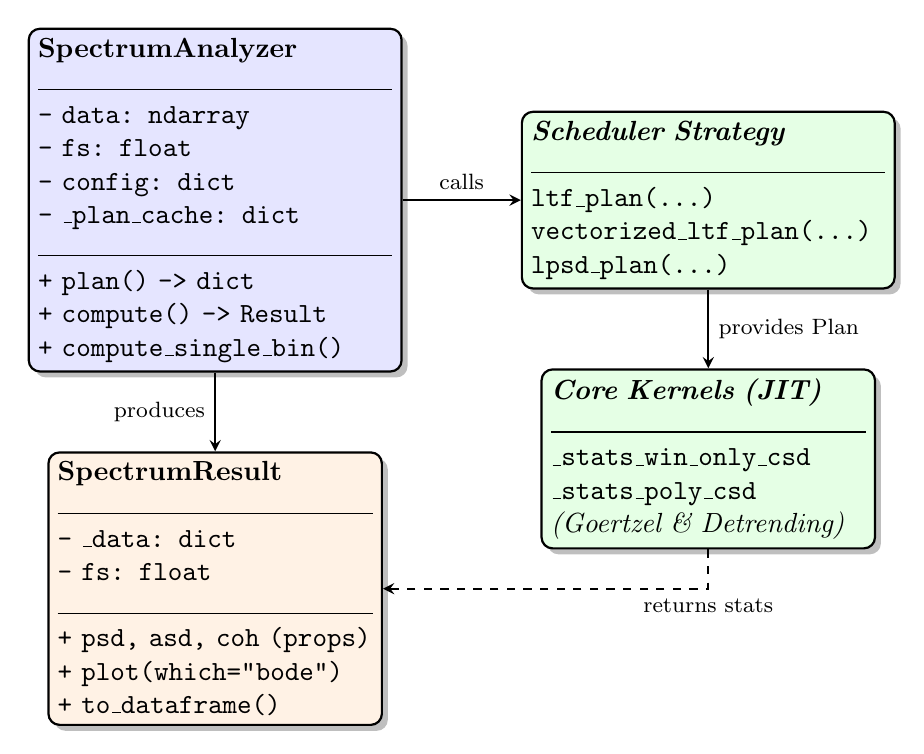
\begin{tikzpicture}[
        node distance=1cm,
        class/.style={rectangle, rounded corners, draw=black, thick, fill=blue!10, minimum height=2.5cm, text width=4.5cm, align=left, drop shadow},
        data/.style={class, fill=orange!10, text width=4cm},
        func/.style={class, fill=green!10, text width=4cm, minimum height=1.5cm},
        arrow/.style={->, thick, >=stealth}
    ]
    
    % Nodes
    \node (analyzer) [class] {
        \textbf{SpectrumAnalyzer} \\
        \hrulefill \\
        \texttt{- data: ndarray} \\
        \texttt{- fs: float} \\
        \texttt{- config: dict} \\
        \texttt{- \_plan\_cache: dict} \\
        \hrulefill \\
        \texttt{+ plan() -> dict} \\
        \texttt{+ compute() -> Result} \\
        \texttt{+ compute\_single\_bin()}
    };

    \node (scheduler) [func, text width=4.5cm, right=1.5cm of analyzer] {
        \textbf{\textit{Scheduler Strategy}} \\
        \hrulefill \\
        \texttt{ltf\_plan(...)} \\
        \texttt{vectorized\_ltf\_plan(...)} \\
        \texttt{lpsd\_plan(...)}
    };

    \node (core) [func, below=1cm of scheduler] {
        \textbf{\textit{Core Kernels (JIT)}} \\
        \hrulefill \\
        \texttt{\_stats\_win\_only\_csd} \\
        \texttt{\_stats\_poly\_csd} \\
        \textit{(Goertzel \& Detrending)}
    };

    \node (result) [data, below=1cm of analyzer] {
        \textbf{SpectrumResult} \\
        \hrulefill \\
        \texttt{- \_data: dict} \\
        \texttt{- fs: float} \\
        \hrulefill \\
        \texttt{+ psd, asd, coh (props)} \\
        \texttt{+ plot(which="bode")} \\
        \texttt{+ to\_dataframe()}
    };

    % Arrows
    \draw[arrow] (analyzer.east) -- node[midway, above, font=\footnotesize] {calls} (scheduler.west);
    \draw[arrow] (scheduler.south) -- node[midway, right, font=\footnotesize] {provides Plan} (core.north);
    \draw[arrow] (analyzer.south) -- node[midway, left, font=\footnotesize] {produces} (result.north);
    \draw[arrow, dashed] (core.south) |- node[midway, below, font=\footnotesize] {returns stats} (result.east);

    \end{tikzpicture}
    \caption{Core architecture of \speckit{}. The \texttt{SpectrumAnalyzer} coordinates the generation of a frequency plan via a Scheduler and the computation of sufficient statistics via the Core Kernels, producing a \texttt{SpectrumResult}.}
    \label{fig:diag_analyzer}
\end{figure*}

\begin{figure*}[t!]
    \centering
    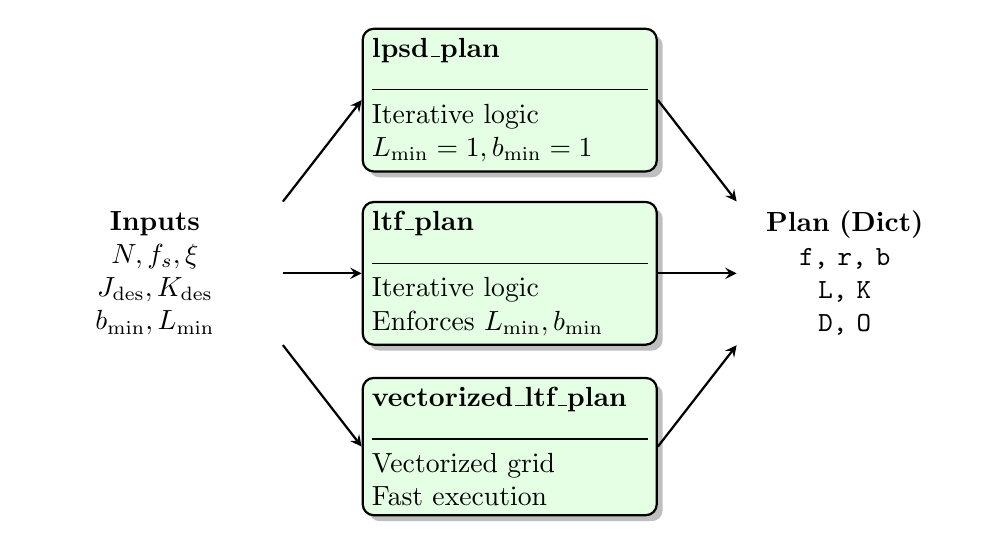
\begin{tikzpicture}[
        node distance=1cm,
        class/.style={rectangle, rounded corners, draw=black, thick, fill=green!10, minimum height=1cm, text width=3.5cm, align=left, drop shadow},
        input/.style={rectangle, draw=none, text width=3cm, align=center},
        arrow/.style={->, thick, >=stealth}
    ]

    \node (inputs) [input] {
        \textbf{Inputs} \\
        $N, f_s, \xi$ \\
        $J_{\text{des}}, K_{\text{des}}$ \\
        $b_{\min}, L_{\min}$
    };

    \node (lpsd) [class, right=1cm of inputs, yshift=2.2cm] {
        \textbf{lpsd\_plan} \\
        \hrulefill \\
        Iterative logic \\
        $L_{\min}=1, b_{\min}=1$
    };

    \node (ltf) [class, right=1cm of inputs] {
        \textbf{ltf\_plan} \\
        \hrulefill \\
        Iterative logic \\
        Enforces $L_{\min}, b_{\min}$
    };

    \node (vect) [class, right=1cm of inputs, yshift=-2.2cm] {
        \textbf{vectorized\_ltf\_plan} \\
        \hrulefill \\
        Vectorized grid \\
        Fast execution
    };

    \node (output) [input, right=1cm of ltf, text width=2.5cm] {
        \textbf{Plan (Dict)} \\
        \texttt{f, r, b} \\
        \texttt{L, K} \\
        \texttt{D, O}
    };

    % Arrows
    \draw[arrow] (inputs.north east) -- (lpsd.west);
    \draw[arrow] (inputs.east) -- (ltf.west);
    \draw[arrow] (inputs.south east) -- (vect.west);
    
    \draw[arrow] (lpsd.east) -- (output.north west);
    \draw[arrow] (ltf.east) -- (output.west);
    \draw[arrow] (vect.east) -- (output.south west);

    \end{tikzpicture}
    \caption{Functional Strategy pattern for Schedulers. All schedulers implement the same interface: transforming configuration constraints into a definitive frequency and segmentation plan.}
    \label{fig:diag_schedulers}
\end{figure*}

\begin{figure*}[t!]
    \centering
    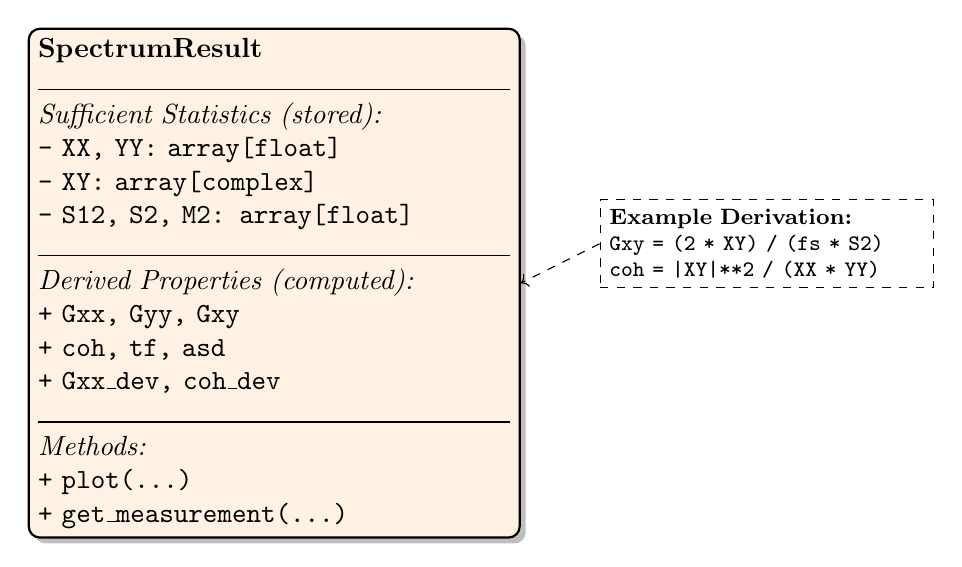
\begin{tikzpicture}[
        node distance=0.5cm,
        class/.style={rectangle, rounded corners, draw=black, thick, fill=orange!10, minimum height=4cm, text width=6cm, align=left, drop shadow},
        note/.style={rectangle, draw=black, dashed, fill=white, text width=4cm, align=left, font=\footnotesize}
    ]

    \node (res) [class] {
        \textbf{SpectrumResult} \\
        \hrulefill \\
        \textit{Sufficient Statistics (stored):} \\
        \texttt{- XX, YY: array[float]} \\
        \texttt{- XY: array[complex]} \\
        \texttt{- S12, S2, M2: array[float]} \\
        \hrulefill \\
        \textit{Derived Properties (computed):} \\
        \texttt{+ Gxx, Gyy, Gxy} \\
        \texttt{+ coh, tf, asd} \\
        \texttt{+ Gxx\_dev, coh\_dev} \\
        \hrulefill \\
        \textit{Methods:} \\
        \texttt{+ plot(...)} \\
        \texttt{+ get\_measurement(...)}
    };

    \node (calc) [note, right=1cm of res, yshift=0.5cm] {
        \textbf{Example Derivation:} \\
        \texttt{Gxy = (2 * XY) / (fs * S2)} \\
        \texttt{coh = |XY|**2 / (XX * YY)}
    };

    \draw[dashed, ->] (calc.west) -- (res.east);

    \end{tikzpicture}
    \caption{Internal structure of the \texttt{SpectrumResult} class. It acts as a lazy evaluator, deriving physical spectral quantities and error estimates on-demand from the raw statistics computed by the kernels.}
    \label{fig:diag_result}
\end{figure*}


\bibliographystyle{elsarticle-num}
\bibliography{bibliography.bib}

\end{document}
